\section{Classifier}

\note{Una vez que estamos en contexto con el área, procedemos a hablar de la implementación del clasificador.}

\subsection{Methodology}
\begin{frame}
    \frametitle{Methodology}

    \begin{itemize}
        \item SVM, kNN, DT, GNB and MNB were tried.
        \item 80\% training and 20\% test.
        \item We used cross validation with the training set to obtain results during the development of the model and the test set for the final results.
    \end{itemize}
\end{frame}

\note{Primero hablamos de la metodología que usamos. Se utilizan las técnicas, SVM, Vecinos más cercanos, Árboles de decisión y dos tipos de clasificadores Naïve Bayes: uno que supone que las probabilidades siguen una distribución gaussiana y otro que supone que siguen una distribución multinomial.

Dividimos el corpus en 80\% entrenamiento y 20\% evaluación. El corpus de evaluación lo dejamos para el final de manera de intentar no sesgarse demasiado a los resultados y que las métricas no sean mentirosas. Mientras se desarrollan las características y el clasificador se utiliza una técnica llamada validación cruzada para evaluar al clasificador. Cuando se quieren estudiar casos puntuales de error, como por ejemplo tweets falsos positivos, se ha partido nuevamente al conjunto de entrenamiento en entrenamiento y evaluación.}

\subsection{Baseline}
\begin{frame}
    \frametitle{Baseline}

    \begin{enumerate}
        \item BoW + MNB

        \item Majority (negative)
    \end{enumerate}

    \begin{center}
        \scriptsize
        \begin{tabular}{ c r r r r r r r }
            & \multicolumn{1}{c}{Precision} & \multicolumn{1}{c}{Recall} & \multicolumn{1}{c}{$F_1$} & \multicolumn{1}{c}{Neg.\ prec.} & \multicolumn{1}{c}{Neg.\ rec.} & \multicolumn{1}{c}{Neg.\ $F_1$} & \multicolumn{1}{c}{Accuracy} \\
            \midrule
            BL1 & \textbf{65.2} & \textbf{82.7} & \textbf{72.9} & \textbf{96.3} & 91.2 & \textbf{93.7} & \textbf{89.7} \\
            \midrule
            BL2 & N/A & 0.0 & N/A & 82.5 & \textbf{100.0} & 90.4 & 82.5 \\
        \end{tabular}
    \end{center}
\end{frame}

\note{Decidimos establecer una línea base para comparar contra las técnicas utilizadas.

El primero de ellos es un modelo llamado Bag of Words, o bolsa de palabras. La idea es transformar cada tweet en un vector de conteos de las palabras que aparecen. Es decir, las características son cada una de las palabras que aparecen en los tweets. Un tweet por ejemplo puede tener la palabra ``mesa'' 2 veces, la palabra ``arte'' una vez y la palabra ``plato'' ninguna vez. Se combina esto con un clasificador Naïve Bayes multinomial.

El segundo es un clasificador mucho más simple. Se limita a predecir en base a la categoría que fue más frecuente en la etapa de entrenamiento. Dice lo que dice la mayoría, en otras palabras. En este caso dice que todo es negativo, No humor, porque observó al rededor de 83\% de negativos al entrenar.}

\note{Acá se muestran los números que se obtuvieron, en donde tenemos la Precisión [señalar], Recall, F1, lo mismo para los negativos y finalmente el acierto. Se puede observar que la primera línea base supera ampliamente a la segunda.}

\subsection{Features}

\begin{frame}
    \frametitle{Features}

    What we are looking for:

    \begin{itemize}
        \item Opposition and negativity
        \item Format
        \item Informality
        \item Focused on people
        \item Recurrent themes in jokes
    \end{itemize}
\end{frame}

\note{Ahora vamos a hablar de las características implementadas. Básicamente buscamos las siguientes cosas: contradicción y negatividad en los tweets, determinado tipo de formato sintáctico, informalidad, que estén centrados en personas y temas recurrentes en chistes.}

\begin{frame}
    \frametitle{Opposition and negativity}
    \framesubtitle{Antonymy}

    \begin{itemize}
        \item WordNet was used
        \item Amount of pairs of antonyms in the tweet:
    \end{itemize}

    \begin{center}
        \[
            Antonymy(tweet) = \frac{|\{antonym\ pairs\}|}{\sqrt{|tweet|}}
        \]
    \end{center}
\end{frame}

\note{Buscando contradicción realizamos la característica Antónimos. Se cuenta la cantidad de pares de antónimos en el tweet en relación a su largo.}

\begin{frame}
    \frametitle{Contradiction and negativity}
    \framesubtitle{Negation}

    \begin{itemize}
        \item Number of ``no'' in the tweet
    \end{itemize}
\end{frame}

\note{Se hace también la característica Negación. Se cuenta la cantidad de ``no'' en el tweet.}

\begin{frame}
    \frametitle{Format}
    \framesubtitle{Dialog}

    \begin{itemize}
        \item If the tweet is a dialog or not
    \end{itemize}
\end{frame}

\note{En cuanto al Formato tenemos primero a Diálogo. Indica si el tweet es un diálogo o no.}

\begin{frame}
    \frametitle{Format}
    \framesubtitle{Links}

    \begin{itemize}
        \item Amount of links
    \end{itemize}
\end{frame}

\note{Luego sigue Links, que cuenta la cantidad de enlaces en el tweet. Como el humor que buscamos debe ser expresado completamente en textos no tendría sentido un enlace a una imagen por ejemplo.}

\begin{frame}
    \frametitle{Format}
    \framesubtitle{Questions-Answers}

    \begin{itemize}
        \item Number of questions followed by answers.
    \end{itemize}
\end{frame}

\note{Preguntas-respuestas: se cuenta la cantidad de preguntas seguidas de respuestas que hay en el tweet.}

\begin{frame}
    \frametitle{Informality}
    \framesubtitle{Exclamation}

    \begin{itemize}
        \item Number of exclamation marks:
    \end{itemize}

    \begin{center}
        \[
            Exclamation(tweet) = \frac{|\{exclamation\ mark\}|}{\sqrt{|tweet|}}
        \]
    \end{center}
\end{frame}

\note{Mirando la Informalidad tenemos por un lado la Exclamación. Cuenta la cantidad de signos de exclamación en relación al largo del tweet. Suele indicar informalidad y potencialmente humor.}

\begin{frame}
    \frametitle{Informality}
    \framesubtitle{Hashtags}

    \begin{itemize}
        \item Number of hashtags
    \end{itemize}
\end{frame}

\note{Hashtags: cuenta la cantidad de hashtags en el tweet.}

\begin{frame}
    \frametitle{Informality}
    \framesubtitle{Out Of Vocabulary words (OOV)}

    \begin{itemize}
        \item Number of OOV words, divided by the total

        \item Multiple features:

        \begin{itemize}
            \item Freeling
            \item Freeling-Google
            \item Freeling-Wiktionary
            \item Wiktionary
        \end{itemize}
    \end{itemize}
\end{frame}

\note{
    Luego sigue OOV\@. Son cuatro características que cuentan la cantidad de palabras fuera del vocabulario en relación al largo del tweet.

    Las distintas combinaciones de diccionarios es debido a ventajas y desventajas de cada uno. \textbf{Freeling} es una herramienta que posee el diccionario más barato de usar que tenemos, porque es offline. Tiene un español más clásico, pero no tiene palabras ``nuevas''. \textbf{Wiktionary} tiene un término medio de todo. Es online, pero no limita su uso, y además tiene algunas palabras modernas. Con \textbf{Google} se pueden obtener muchas palabras ``nuevas'' (como iPhone) y también detección de errores ortográficos, pero limita su uso.
}

\begin{frame}
    \frametitle{Informality}
    \framesubtitle{Uppercase words}

    \begin{itemize}
        \item Amount of words totally in uppercase:
    \end{itemize}

    \begin{center}
        \[
            UppercaseWords(tweet) = \frac{|\{uppercase\ words\}|}{\sqrt{|tweet|}}
        \]
    \end{center}
\end{frame}

\note{Palabras mayúsculas: se cuenta la cantidad de palabras totalmente en mayúsculas en relación a la cantidad de palabras del tweet. Cuando hay palabras en mayúsculas es como si estuvieran gritando en el tweet, lo cual da informalidad y potencialmente humor, ya que creemos que el humor suele ser informal.}

\begin{frame}
    \frametitle{Informality}
    \framesubtitle{Non-Spanish words}

    \begin{itemize}
        \item Number of words that have letters out of the Spanish alphabet, normalizing with respect to the total.
    \end{itemize}
\end{frame}

\note{Palabras no españolas: se cuenta la cantidad de palabras que contienen caracteres fuera del alfabeto español, normalizando según el total. Se fija por la presencia de caracteres raros que indican, de vuelta, informalidad.}

\begin{frame}
    \frametitle{Focused on people}
    \framesubtitle{First and Second person}

    \begin{itemize}
        \item We look for words inflexed in first person and the same for second person.
    \end{itemize}
\end{frame}

\note{En cuanto a Orientación en personas tenemos Primera persona y Segunda persona, dos características. La primera busca palabras en primera persona, ya sean verbos, sustantivos, adjetivos; como ``hago'' o ``yo''. La segunda busca palabras como ``tú'' o ``haces''.}

\begin{frame}
    \frametitle{Recurrent themes in jokes}
    \framesubtitle{Thematic distance}

    \begin{itemize}
        \item Similarity to a joke category from Chistes.com or to a Wikipedia sentence.

        \item BoW + MNB

        \item Categories:

        \begin{itemize}
            \item Short jokes
            \item Riddles
            \item Animals
            \item Ethnic jokes
            \item Others
        \end{itemize}
    \end{itemize}
\end{frame}

\note{En Temas recurrentes en chistes tenemos primero Distancia temática. La idea es fijarse qué cercanía tiene un tweet a una categoría de chistes de la página Chistes.com, contrastando con oraciones de Wikipedia. Se toman las 5 categorías que más tienen chistes, armando 5 características entonces. Cada una arma un subclasificador, utilizando el modelo Bag of Words con Naïve Bayes multinomial, así como la primera línea base, tomando como características a los conteos de cada palabra. Se obtiene entonces una categoría (chiste de Chistes.com u oración de Wikipedia) y a la vez un número que indica la probabilidad de acercarse a una categoría, que es particularmente devuelto por Naïve Bayes.}

\begin{frame}
    \frametitle{Recurrent themes in jokes}
    \framesubtitle{Sexual slang}

    \begin{itemize}
        \item We built a sexual slang dictionary bootstrapping from Twitter and curating manually.

        \item Multiset intersection:
    \end{itemize}

    \begin{center}
        \[
            SexualSlang(tweet) = \frac{|tweet \cap DIC_{SS}|}{\sqrt{|tweet|}}
        \]
    \end{center}
\end{frame}

\note{Jerga sexual. Se arma un diccionario de jerga sexual. Primero intuitivamente. Luego se refuerza mediante una técnica, llamada Bootstrapping, en la que se buscan tweets que aparezcan las palabras de este primer diccionario y nos fijamos qué palabras más co-ocurren con ellas, agrandando el diccionario.

Luego nos fijamos la cantidad de palabras de los tweets que pertenecen a este diccionario, en relación al total de palabras del tweet.}

\begin{frame}
    \frametitle{Recurrent themes in jokes}
    \framesubtitle{Keywords}

    \begin{itemize}
        \item List of frequent words in jokes.
        \item Multiset intersection:
    \end{itemize}

    \begin{center}
        \[
            Keywords(tweet) = \frac{|tweet \cap DIC_{KW}|}{\sqrt{|tweet|}}
        \]
    \end{center}
\end{frame}

\note{En Palabras clave se arma un diccionario de palabras comunes en chistes empíricamente, como ``mamá'' y ``Jaimito'', y luego se procede de manera similar a la característica anterior con el diccionario.}

\begin{frame}
    \frametitle{Recurrent themes in jokes}
    \framesubtitle{Animal presence}

    \begin{itemize}
        \item A list of animals from the jokes in Chistes.com is formed

        \item Multiset intersection:

        \begin{center}
            \[
                AnimalPresence(tweet) = \frac{|tweet \cap DIC_A|}{\sqrt{|tweet|}}
            \]
        \end{center}
    \end{itemize}
\end{frame}

\note{Se conforma una lista de animales a partir de las palabras que aparecen en los chistes de animales de Chistes.com. Luego se procede como antes, contando la ocurrencia de palabras de un tweet en el diccionario y normalizando según la cantidad de palabras del tweet.}

\subsection{Feature selection}
\begin{frame}[allowframebreaks]
    \frametitle{Feature selection}

    \begin{itemize}
        \item ExtraTrees is used to rank them first, just to see.

        \item Then Recursive Feature Elimination is used to restrict to relevant only.
    \end{itemize}

    \note{Luego se procede a seleccionar las características. La idea es quitar aquellas irrelevantes o redundantes. Se procede primero utilizando una técnica llamada ExtraTrees, que genera una cantidad fija de Árboles de decisión aleatorios, y se fija qué características discriminan mejor. Se utiliza para hacer un ranking de las características.

    Luego se utiliza la Eliminación recursiva de atributos para seleccionar finalmente las características. La técnica procede a quitar las características más irrelevantes una a una y fijarse con qué número se obtiene mejor acierto.}

    \framebreak{}

    ExtraTrees:

    \begin{center}
        \tiny
        \begin{tabular}{ c r }
            \multicolumn{1}{c}{\textbf{Característica}} & \multicolumn{1}{c}{\textbf{Valor}} \\
            CLASS & 74.05 \\
            Diálogo & 10.86 \\
            Distancia temática: Otros\ldots & 03.07 \\
            Distancia temática: Atlantes & 02.65 \\
            Distancia temática: Chistes cortos & 02.53 \\
            Preguntas-respuestas & 01.98 \\
            Distancia temática: Adivinanzas & 0.95 \\
            Distancia temática: Animales & 0.87 \\
            Palabras clave & 0.57 \\
            Exclamación & 0.57 \\
            Hashtags & 0.55 \\
            Links & 0.54 \\
            Primera persona & 0.21 \\
            Segunda persona & 0.15 \\
            OOV Freeling & 0.08 \\
            Palabras mayúsculas & 0.06 \\
            ALEATORIA & 0.06 \\
            Jerga sexual & 0.06 \\
            Negación & 0.05 \\
            OOV Wiktionary & 0.04 \\
            OOV Freeling Wiktionary & 0.03 \\
            Presencia de animales & 0.03 \\
            OOV Freeling Google & 0.03 \\
            Antónimos & 0.02 \\
            Palabras no españolas & 0.00 \\
        \end{tabular}
    \end{center}

    \note{Se obtiene esta tabla. Se introducen dos características ficticias para comparar. La primera es CLASE, una característica que sabe exactamente si un tweet es humorístico o no, sabe la solución. Por otro lado está ALEATORIA, que tiene un valor aleatorio.

    Observar que por ejemplo Diálogo, Preguntas-respuestas y las de Distancia temática son las características que más discriminan al humor. Ver por otro lado que características como las de OOV, Antónimos y Jerga sexual resultan ser peores que el azar.}

    \framebreak{}

    Recursive Feature Elimination:

    \begin{center}
        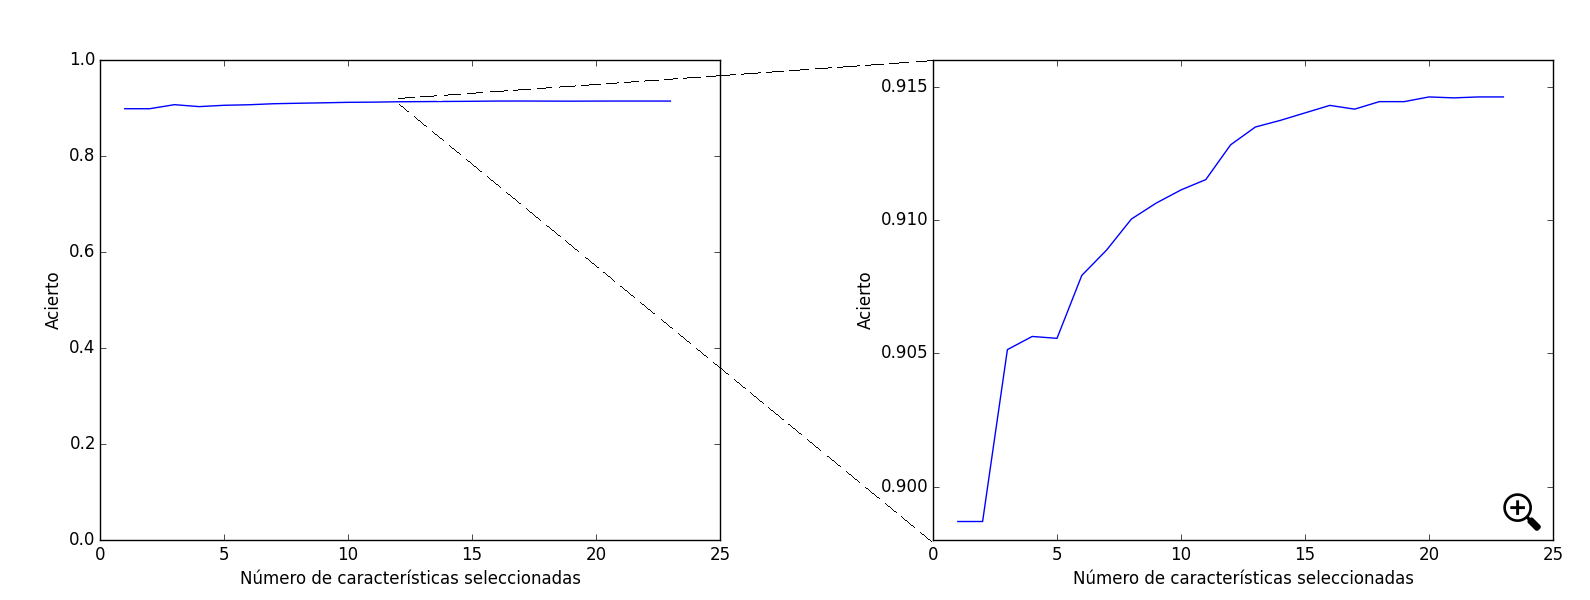
\includegraphics[height=4cm]{rfe.png}

        \vspace{1cm}

        Negation, Non-Spanish words and Antonymy are dropped.
    \end{center}
\end{frame}

\note{Esta es la gráfica resultado que se obtiene de la Eliminación recursiva de atributos. El máximo acierto se obtiene al eliminar tres, pero observar que la variación total del acierto es muy poca, inclusive para el máximo.

Finalmente se descartan entonces Negación, Palabras no españolas y Antónimos.

A continuación mi compañero Matías va a proceder a mostrar los resultados obtenidos.}

\subsection{Obtained results}
\begin{frame}
    \frametitle{Obtained results}

    \begin{center}
        \scriptsize
        \begin{tabular}{ c r r r r r r r }
            & \multicolumn{1}{c}{Precision} & \multicolumn{1}{c}{Recall} & \multicolumn{1}{c}{$F_1$} & \multicolumn{1}{c}{Neg.\ prec.} & \multicolumn{1}{c}{Neg.\ rec.} & \multicolumn{1}{c}{Neg.\ $F_1$} & \multicolumn{1}{c}{Accuracy} \\
            \midrule
            LB1 & \textbf{61.7} & \textbf{84.6} & \textbf{71.4} & \textbf{96.6} & 89.2 & 71.4 & \textbf{88.5} \\
            \midrule
            LB2 & N/A & 0.0 & N/A & 83.0 & \textbf{100.0} & \textbf{90.7} & 83.0 \\
            \midrule
            \midrule
            SVM & 83.6 & 68.9 & \textbf{75.5} & 93.8 & 97.2 & \textbf{95.5} & \textbf{92.5} \\
            \midrule
            DT & 66.5 & 67.5 & 67.0 & 93.3 & 93.0 & 93.2 & 88.9 \\
            \midrule
            GNB & 57.5 & \textbf{78.2} & 66.3 & \textbf{95.2} & 88.2 & 91.5 & 86.5 \\
            \midrule
            MNB & \textbf{84.8} & 60.0 & 70.3 & 92.3 & \textbf{97.8} & 95.0 & 91.4 \\
            \midrule
            KNN & 81.3 & 66.3 & 73.0 & 93.4 & 96.9 & 95.1 & 91.7 \\
        \end{tabular}

        \begin{center}
            Best technique: \textbf{SVM}
        \end{center}

        \begin{tabular}{ c r r }
            \textbf{are/classified} & Positive & Negative \\
            \midrule
            Positive & 842 & 381 \\
            \midrule
            Negative & 165 & 5805 \\
        \end{tabular}
    \end{center}
\end{frame}

\subsection{Other analysis}

\subsubsection{Banned tweets}
\begin{frame}
    \frametitle{Banned tweets}

    \begin{itemize}
        \item The classifier is biased against tweets with explicit content.
        \item They were annotated by hand (303 tweets)
        \item There's a little improvement:
        \begin{center}
            \scriptsize
            \begin{tabular}{ c r r r r r r r }
                \textbf{SVM} & \multicolumn{1}{c}{Precision} & \multicolumn{1}{c}{Recall} & \multicolumn{1}{c}{$F_1$} & \multicolumn{1}{c}{Neg.\ prec.} & \multicolumn{1}{c}{Neg.\ rec.} & \multicolumn{1}{c}{Neg.\ $F_1$} & \multicolumn{1}{c}{Accuracy} \\
                \midrule
                Before & 83.6 & 68.9 & 75.5 & \textbf{93.8} & \textbf{97.2} & \textbf{95.5} & \textbf{92.5} \\
                \midrule
                After & \textbf{84.0} & \textbf{69.6} & \textbf{76.1} & 93.7 & \textbf{97.2} & 95.4 & 92.3 \\
            \end{tabular}
        \end{center}
        \item A new study of feature importance reveals that Sexual slang doesn't change: more variety than what's related to Sexual slang was added by doing this.
    \end{itemize}
\end{frame}

\subsubsection{Restricted to humorous accounts}
\begin{frame}
    \frametitle{Restricted to humorous accounts}

    \begin{itemize}
        \item It's a harder task.
        \item Good results anyway:

        \begin{center}
            \scriptsize
            \begin{tabular}{ c r r r r r r r }
                & \multicolumn{1}{c}{Precision} & \multicolumn{1}{c}{Recall} & \multicolumn{1}{c}{$F_1$} & \multicolumn{1}{c}{Neg.\ prec.} & \multicolumn{1}{c}{Neg.\ rec.} & \multicolumn{1}{c}{Neg.\ $F_1$} & \multicolumn{1}{c}{Accuracy} \\
                \midrule
                SVM & \textbf{81.9} & 73.8 & 77.6 & 78.5 & \textbf{85.4} & \textbf{81.8} & \textbf{79.9} \\
                \midrule
                DT & 74.5 & 75.5 & 75.0 & 72.2 & 71.1 & 71.7 & 74.1 \\
                \midrule
                GNB & 78.7 & 78.6 & \textbf{78.6} & 76.1 & 76.3 & 76.2 & 77.5 \\
                \midrule
                MNB & 68.5 & \textbf{85.5} & 76.1 & \textbf{83.3} & 64.6 & 72.9 & 74.6 \\
                \midrule
                KNN & 79.2 & 73.0 & 76.0 & 77.4 & 82.9 & 80.1 & 78.1 \\
            \end{tabular}
        \end{center}
    \end{itemize}
\end{frame}

\subsubsection{Humor vs.\ the non-humorous account types}
\begin{frame}
    \frametitle{Humor vs.\ the non-humorous account types}

    \begin{center}
        \scriptsize
        \begin{tabular}{ c r r r r r r r }
            \textbf{SVM} & \multicolumn{1}{c}{Precision} & \multicolumn{1}{c}{Recall} & \multicolumn{1}{c}{$F_1$} & \multicolumn{1}{c}{Neg.\ prec.} & \multicolumn{1}{c}{Neg.\ rec.} & \multicolumn{1}{c}{Neg.\ $F_1$} & \multicolumn{1}{c}{Accuracy} \\
            \midrule
            News & \textbf{97.0} & \textbf{95.2} & \textbf{96.1} & \textbf{97.0} & \textbf{98.1} & \textbf{97.5} & \textbf{97.0} \\
            \midrule
            Phil.\ thoughts & 95.0 & 83.0 & 88.6 & 84.0 & 95.3 & 89.3 & 88.9 \\
            \midrule
            Curiosities & 94.6 & 83.7 & 88.9 & 88.2 & 96.3 & 92.1 & 90.7 \\
        \end{tabular}
    \end{center}
\end{frame}
